% Options for packages loaded elsewhere
\PassOptionsToPackage{unicode}{hyperref}
\PassOptionsToPackage{hyphens}{url}
\PassOptionsToPackage{dvipsnames,svgnames*,x11names*}{xcolor}
%
\documentclass[
]{article}
\usepackage{lmodern}
\usepackage{amssymb,amsmath}
\usepackage{ifxetex,ifluatex}
\ifnum 0\ifxetex 1\fi\ifluatex 1\fi=0 % if pdftex
  \usepackage[T1]{fontenc}
  \usepackage[utf8]{inputenc}
  \usepackage{textcomp} % provide euro and other symbols
\else % if luatex or xetex
  \usepackage{unicode-math}
  \defaultfontfeatures{Scale=MatchLowercase}
  \defaultfontfeatures[\rmfamily]{Ligatures=TeX,Scale=1}
\fi
% Use upquote if available, for straight quotes in verbatim environments
\IfFileExists{upquote.sty}{\usepackage{upquote}}{}
\IfFileExists{microtype.sty}{% use microtype if available
  \usepackage[]{microtype}
  \UseMicrotypeSet[protrusion]{basicmath} % disable protrusion for tt fonts
}{}
\makeatletter
\@ifundefined{KOMAClassName}{% if non-KOMA class
  \IfFileExists{parskip.sty}{%
    \usepackage{parskip}
  }{% else
    \setlength{\parindent}{0pt}
    \setlength{\parskip}{6pt plus 2pt minus 1pt}}
}{% if KOMA class
  \KOMAoptions{parskip=half}}
\makeatother
\usepackage{xcolor}
\IfFileExists{xurl.sty}{\usepackage{xurl}}{} % add URL line breaks if available
\IfFileExists{bookmark.sty}{\usepackage{bookmark}}{\usepackage{hyperref}}
\hypersetup{
  pdftitle={Hausübung SDA Chocolate},
  pdfauthor={Dozent: Dr.~Matthias Templ ZHAW IDP},
  colorlinks=true,
  linkcolor=red,
  filecolor=Maroon,
  citecolor=Blue,
  urlcolor=Blue,
  pdfcreator={LaTeX via pandoc}}
\urlstyle{same} % disable monospaced font for URLs
\usepackage[margin=1in]{geometry}
\usepackage{graphicx}
\makeatletter
\def\maxwidth{\ifdim\Gin@nat@width>\linewidth\linewidth\else\Gin@nat@width\fi}
\def\maxheight{\ifdim\Gin@nat@height>\textheight\textheight\else\Gin@nat@height\fi}
\makeatother
% Scale images if necessary, so that they will not overflow the page
% margins by default, and it is still possible to overwrite the defaults
% using explicit options in \includegraphics[width, height, ...]{}
\setkeys{Gin}{width=\maxwidth,height=\maxheight,keepaspectratio}
% Set default figure placement to htbp
\makeatletter
\def\fps@figure{htbp}
\makeatother
\setlength{\emergencystretch}{3em} % prevent overfull lines
\providecommand{\tightlist}{%
  \setlength{\itemsep}{0pt}\setlength{\parskip}{0pt}}
\setcounter{secnumdepth}{-\maxdimen} % remove section numbering
\usepackage{pdfpages}
\usepackage{amsmath}
\usepackage{placeins}
\newlength{\cslhangindent}
\setlength{\cslhangindent}{1.5em}
\newenvironment{cslreferences}%
  {}%
  {\par}

\title{Hausübung SDA Chocolate}
\author{Dozent: Dr.~Matthias Templ ZHAW IDP}
\date{Autoren: Philipp Rieser \& Pascal Simon Bühler WI17t 23-4-2021 ZH}

\begin{document}
\maketitle

\captionsetup[figure]{name=Abbildung}
\captionsetup[table]{name=Tabelle}

\hypertarget{zweck-der-uxfcbung}{%
\section{Zweck der Übung}\label{zweck-der-uxfcbung}}

Diese Aufgabe hat zum Zweck einen Artikel etwas genauer unter die Lupe
zu nehmen und auf Stimmigkeit zu überprüfen. Dazu werden die im Artikel
getroffenen Aussagen basierend auf der zugrundeliegenden Studie
analysiert.

\hypertarget{schoko-milch-gegen-normale-sportgetruxe4nke} mehr als vorher auf der Hantelbank, während die Sportler,
die das kommerzielle Sportgetränk tranken, ihre Kraft beim Bankdrücken
um etwa \textbf{3,2\%} verringerten. Das ist ein Nettounterschied von
\textbf{6,7\%} für diejenigen, die Schokoladenmilch im Vergleich zu
einem kommerziellen Sportgetränk tranken.

Beide Gruppen zeigten eine Verbesserung bei Kniebeugen, aber die
Schokomilch-Trinker zeigten mehr, sie hoben \textbf{15\%} mehr Gewicht
als vorher - während die kommerziellen Sportgetränketrinker nur
\textbf{8\%} mehr hoben. Das ist fast \textbf{doppelt} so viel
Kraftzuwachs bei den Schokomilch-Trinkern.\(\ _{1}\)

Weiter beschreibt Herr Chesire dass der Unterschied von \emph{normalen
Sportgetränken} darin besteht, dass dem Sportgetränk das Protein fehle
wobei Milch zwei Arten von hochwertigem Protein enthält Kasein und
Molkeprotein. Weiter wird beschrieben, dass Milch pro Unze (28.35g)
jeweils ein Gramm Protein enthält welches in Kombination mit den
Kohlenhydraten aus der Schokomilch ein ideales Verhätnis zur
Muskelerholung enthält.\(\ _{2}\)

Hinzufügend wird gesagt dass Schokomilch ein kostengünstiges Getränk ist
zur Rehydration, Auffüllen der glykämischen Speicher und dem
Muskelaufbau. Weitere Studien könnten herausfinden, wie andere Faktoren
die UT-Ergebnisse beeinflusst haben - Dinge wie die Technik oder die
Lebensmittel, die die Sportler zu Hause essen. Die Studie unterstützt
jedoch Schokoladenmilch als Regenerationsergänzung für Jugendliche, die
an intensivem Training teilnehmen.\(\ _{2}\)

Desweiteren ist die Studie verlinkt.

\(\ _{1}\) \emph{Original aus dem Englischen ins Deutsche übersetzt
{[}1{]}} \(\ _{2}\) \emph{Sinngemäss aus dem Englischen ins Deutsche
übersetzt {[}1{]}}

\newpage

\hypertarget{informationen-zur-studie-und-dem-artikel}{%
\section{Informationen zur Studie und dem
Artikel}\label{informationen-zur-studie-und-dem-artikel}}

Die Studie {[}2{]} wurde an der University of Texas at Austin USA
durchgeführt und ist finanziert von Dairy Max einem Verband von
Milchprodukte Vertretern. Der Artikel {[}1{]} ist auf der Website von
Dairy Max erschienen und wurde von Andy Chesire welcher ebenfalls an der
Studie beteiligt war, geschrieben.

\hypertarget{beschreibung-der-studie}{%
\subsection{Beschreibung der Studie}\label{beschreibung-der-studie}}

Ziel der Studie ist es den Effekt zu untersuchen ob Schokoladenmilch
einen Unterschied macht zu normalen Sportgetränken bei heranwachsenden
Athleten. 103 heranwachsenden Athleten (Frauen und Männer) wurden
während eines 7 wöchigen Sommer Trainingsprogrammes entweder CM
(Schokoladenmilch) oder CHO (Kohlenhydrate) direkt nach dem Training
verabreicht. In der ersten Woche sowie in der letzen Woche wurden Kraft
und Ausdauertests durchgeführt. Wobei 5 Wochen lang 4 Tage die Woche
trainiert wurde. Die Trainings Einheiten bestanden aus jeweils 1 Stunde
Kraft und 1 Stunde Ausdauertraining pro Trainingstag, wobei direkt nach
der letzten Trainingseinheit das Getränk verabreicht wurde.

\begin{figure}

{\centering 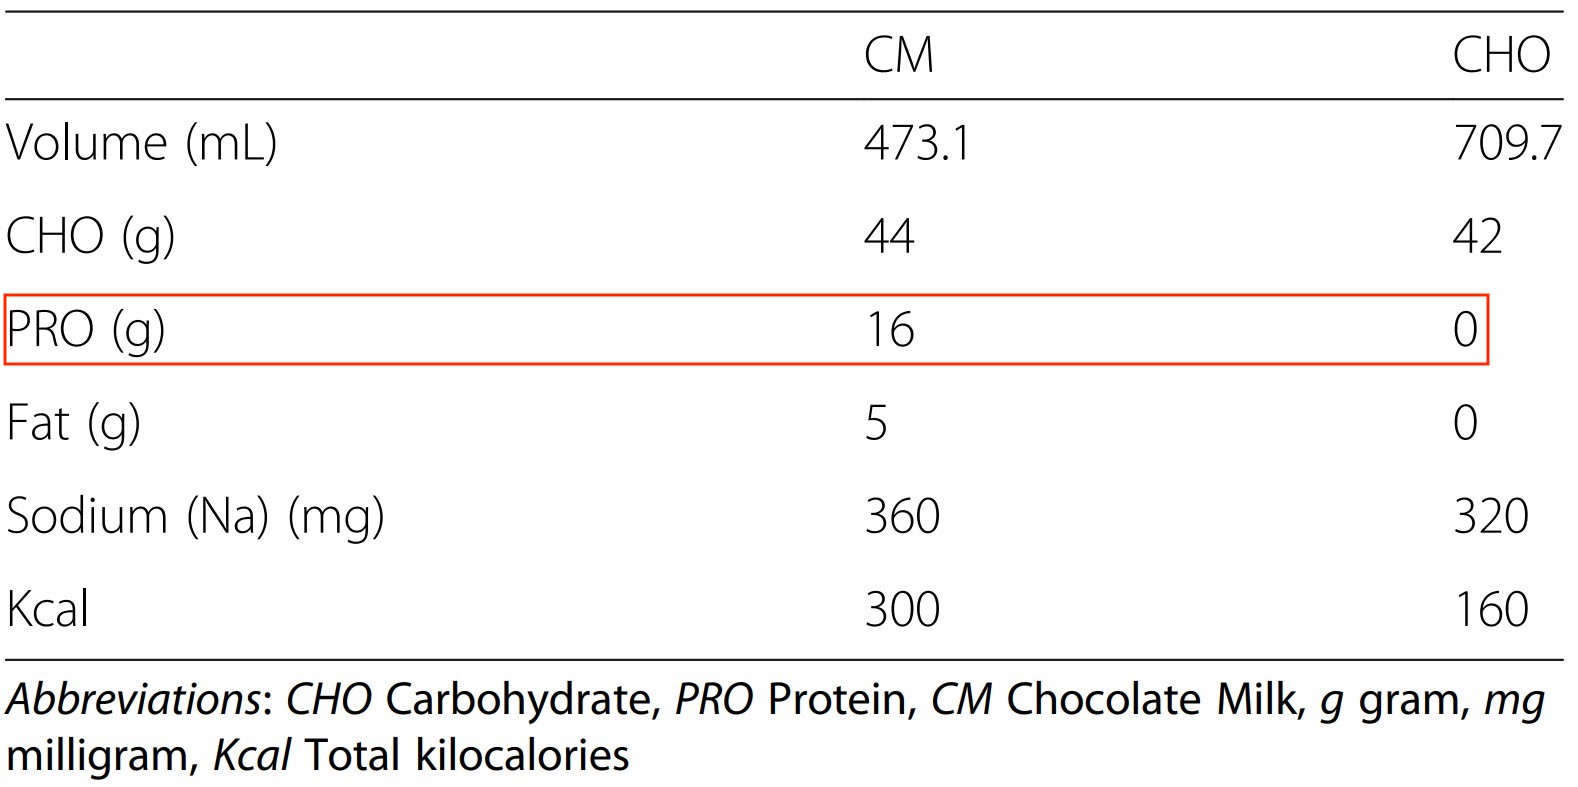
\includegraphics[width=0.6\linewidth]{makronaehrstoffe} 

}

\caption{Makronährstoffe verabreichte Getränke}\label{fig:makro}
\end{figure}

\hypertarget{grundgesamtheit}{%
\subsection{Grundgesamtheit}\label{grundgesamtheit}}

Die Grundgesamheit sind alle jugendlichen High School Sportler in den
USA. Gemass {[}3{]} waren in der Saison 2016-2017 7'963'535 jugendliche
Sportler aktiv.

\hypertarget{auswahlrahmen}{%
\subsection{Auswahlrahmen}\label{auswahlrahmen}}

Der Auswahlrahmen soll die Grundgesamtheit möglichst gut repräsentieren.
In der dieser Studie wurden lediglich Teilnehmer eines
Sommer-Traininglagers einer grossen westlichen High School ausgewählt.
Es ist fraglich ob rein nur die Testteilnehmer einer Schule
repräsentativ für sämtliche High School Sportler der USA sein sollen.
Andere Schulen haben womöglich eine ganz andere Verteilung an
sportlichen Schüler. In der Studie wird der Einsatz von Schokoladenmilch
für die Erholungsphase getestet, ist nun der Anteil an Personen die eine
Unverträglichkeit gegen Laktose haben sehr hoch, könnte es sein, dass
man auf andere Lösungen kommen würde und man hier allenfalls ein
verzerrtes Bild haben.

Es ist nicht ganz klar, ob der Auswahlrahmen die Grundgesamtheit adäquat
repräsentiert.

\hypertarget{stichprobendesign}{%
\subsection{Stichprobendesign}\label{stichprobendesign}}

Es haben 131 Teilnehmer des Trainingslagers an der Studie teilgenommen.
Davon haben 103 die Studie beendet. Somit hat die Studie 28
Nonresponses. In der Studie wird nicht erläutert was mit den fehlenden
Werten gemacht wurde.

Die Teilnehmer wurden bereits von den Trainern des Traningslagers in 3
Gruppen aufgeteilt. Die erste Gruppe mit nur weiblichen Teilnehemer im
Alter zwischen 13-17 Jahren. Die zweite Gruppe mit männlichen Teilnehmer
im Alter zwischen 13-15 Jahren und die dritte Gruppe mit männlichen
Teilnehmer zwischen 15-17 Jahren.

Es ist nicht klar, ob die Stichprobe aus der gesamten Anzahl an
Teilnehmenern gezogen wurde, oder ob auf eine bestimmte stratifizierte
Art aus den Gruppen gezogen wurde (also ob gleichmässig gezogen wurde
oder je nach relativen Häufigkeiten in den Gruppen).

Man weiss auch nicht, wieviele Nonresponses aus welcher Gruppe stammen.

\hypertarget{stichprobe}{%
\subsection{Stichprobe}\label{stichprobe}}

Die Studie beschreibt, dass sie die Teilnehmenden zufällig in die 2
Kategorien CM und CHO einteilen. Eine genaue Auflistung der gekreuzten
Variablen (Gruppierungen) zu den beiden Testkategorien wird in der
Studie nicht aufgezeigt, jedoch beschreiben die Herausgeber der Studie,
dass keine statistische Unterschiede in den Gruppierungen festzustellen
wären.

Zusätzlich mussten die Teilnehmer der Studie folgende Eigenschaften
erfüllen:

\begin{itemize}
\tightlist
\item
  müssen Englisch sprechen
\item
  sollen per Textnachricht erreichbar sein (Besitz eines Handys)
\item
  keine Verletzungen aufweisen
\item
  keine mentale oder physische Behinderungen
\item
  keine Allergien (auf Stoffe welche die verabreichten Getränke
  beinhalten) oder laktoseintoleranz.
\end{itemize}

Gemäss {[}4{]} sind ca 30\% der erwachsenen Leute in den USA Laktose
intolerant. Bei gewissen Bevölkerungsgruppen liegt die Laktoseintoleranz
sogar weit höher zum Beispiel Personen aus dem asiatischen Raum mit bis
zu 90\%. Diese Zahlen wurden zwar für erwachsene Menschen erhoben,
jedoch schliessen sie eine nicht unerheblichen Teil aus der
Grundgesamheit aus. Somit könnte das Ausschliessen von Menschen mit
einer Laktose-Unverträglichkeit eine Verzerrung auf die Grundgesamtheit
aufweisen. Womöglich hätte die Einnahme von Schokoladenmilch bei einer
Laktoseintolarenten Person zu einem positiven Effekt auf das physische
Training

\begin{figure}

{\centering 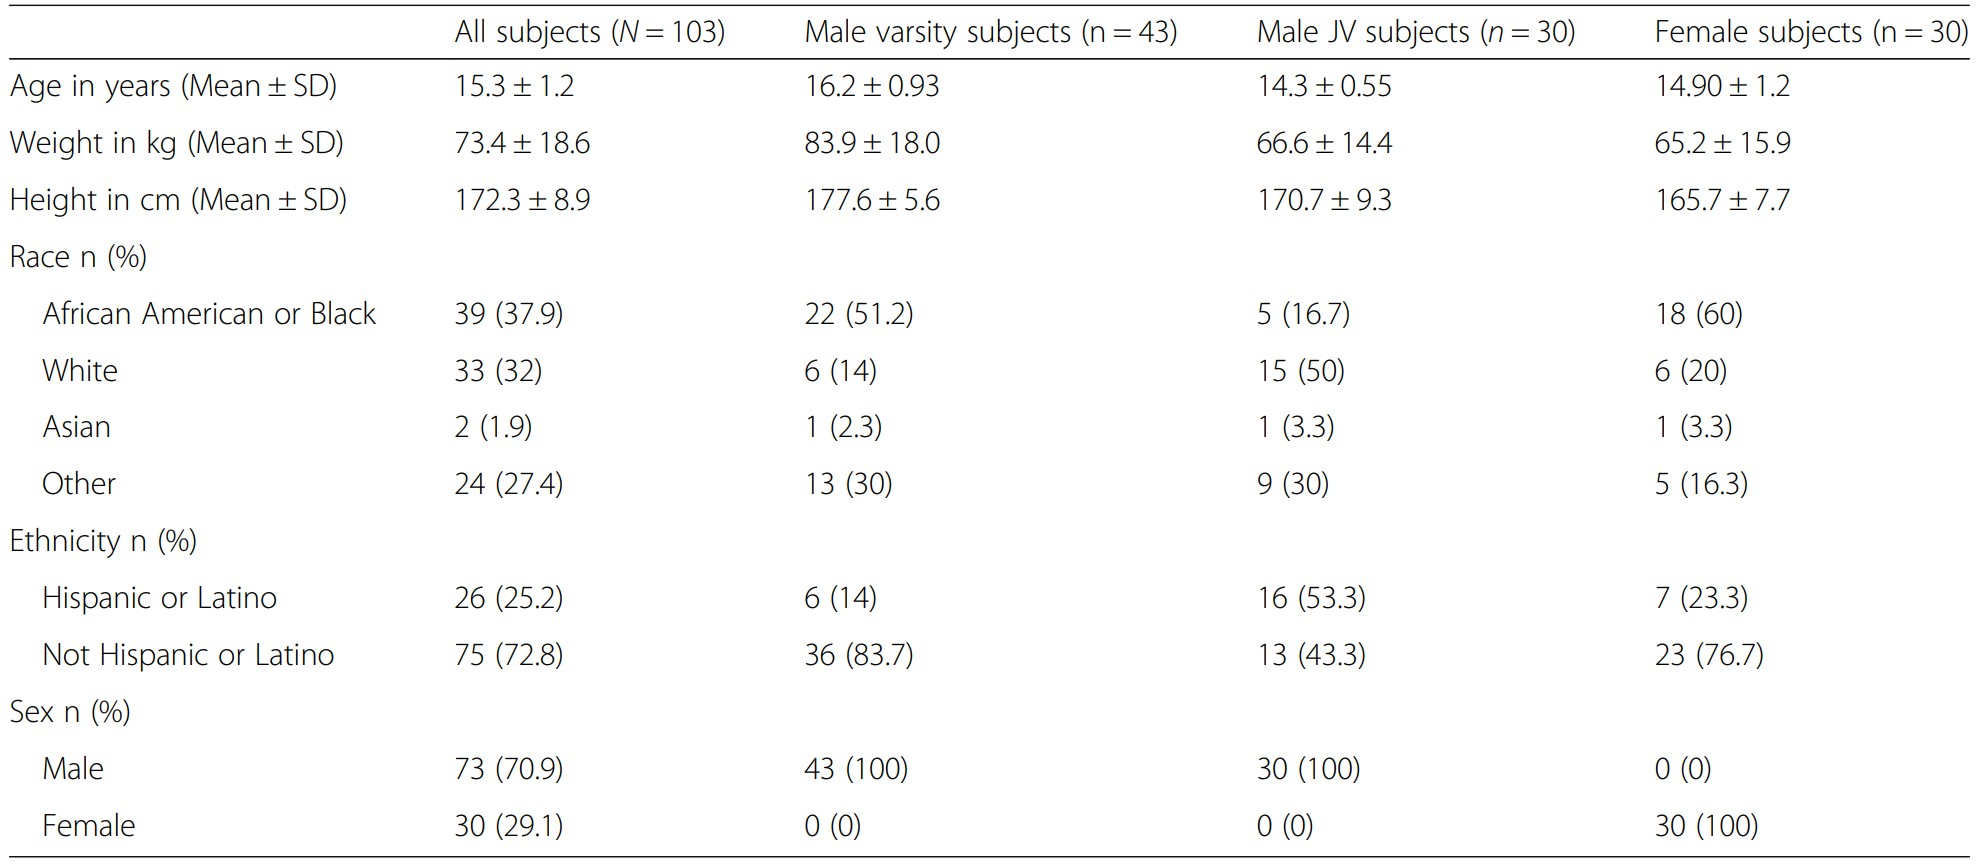
\includegraphics[width=1\linewidth]{subjects} 

}

\caption{Subjects}\label{fig:subjects}
\end{figure}

\hypertarget{versuchsaufbau}{%
\subsection{Versuchsaufbau}\label{versuchsaufbau}}

\hypertarget{resultate}{%
\subsection{Resultate}\label{resultate}}

\begin{figure}

{\centering 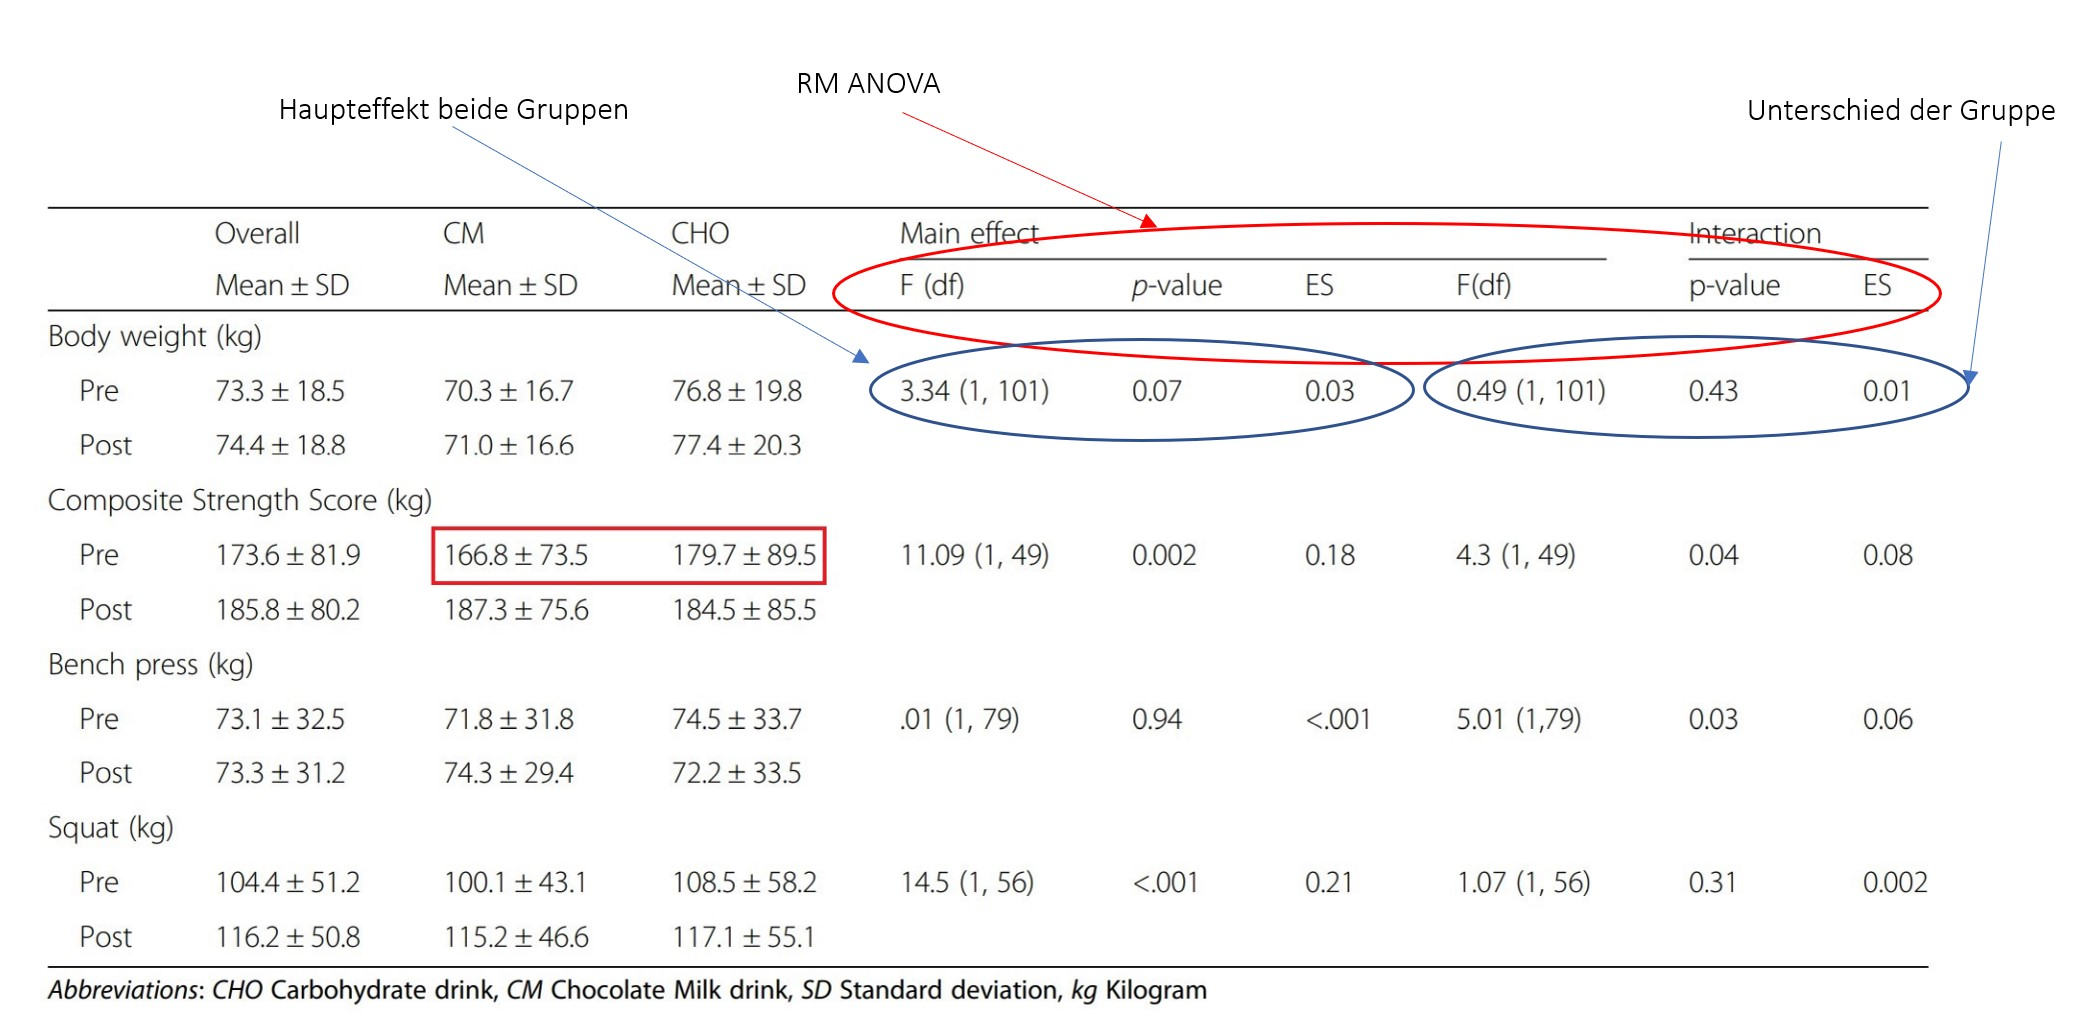
\includegraphics[width=1\linewidth]{results} 

}

\caption{Results}\label{fig:results}
\end{figure}

-Unterschiede in den Stichproben selbst CHO - CM mehr als 10 kg
unterschied vorher, trainings effekt nicht linear

Auf den ersten Blick erkennt man in den samples für CHO und CM grosse
Unterschiede.

Bei Squad unterscheidet sich der Mittelwert sogar um mehr als 10kg. Um
statistisch zu urteilen, wenden wir den z -test an und schauen ob die
Unterschiede signifikant sind.

Da nicht angegeben ist wieviele Teilnehmer welche Beverage bekommen
haben, (In der Studie wird beschrieben zufällige Zuteilung) nehmen wird
die Zuteilung 51/52 an für die Hypothesentests.

\(z=\frac{x1-x2}{ \frac{sd1^{2}}{n1} + \frac{sd2^{2}}{n2} }\)

mit:

\(H_{0} : \mu_{1} = \mu_{2}\) und \(H_{1} : \mu_{1} \neq \mu_{2}\)

\newpage

\hypertarget{abkuxfcrzungen}{%
\subsection{Abkürzungen}\label{abkuxfcrzungen}}

\begin{itemize}
\tightlist
\item
  CHO = Kohlenhydrathaltiger Nahrungsergänzungsmittel
\item
  CM = Schokoladenmilch
\end{itemize}

\hypertarget{referenzen}{%
\subsection{Referenzen}\label{referenzen}}

\hypertarget{refs}{}
\begin{cslreferences}
\leavevmode\hypertarget{ref-article}{}%
{[}1{]} A. Chesire, ``NEW research: CHOCOLATE milk vs. REGULAR sports
drink.''
\url{https://www.dairydiscoveryzone.com/blog/new-research-chocolate-milk-vs-regular-sports-drink}
(accessed Aug. 22, 2017).

\leavevmode\hypertarget{ref-study}{}%
{[}2{]} P. A. C. Katelyn A. Born Erin E. Dooley and J. B. Bartholomew,
\emph{Chocolate milk versus carbohydrate supplements in adolescent
athletes: A field based study}. online: Born et al. Journal of the
International Society of Sports Nutrition, 2019, p. 9.

\leavevmode\hypertarget{ref-survey}{}%
{[}3{]} N. F. of State High School Associations, \emph{Highschool
athletics participation survey}. online: National Federation of State
High School Associations, pp. p. 53--71.

\leavevmode\hypertarget{ref-lactose}{}%
{[}4{]} N. I. R. Center, \emph{Lactose intolerance information for
health care providers}. U.S. DEPARTMENT OF HEALTH AND HUMAN SERVICES, p.
2.
\end{cslreferences}

\end{document}
